\documentclass[pdflatex,sn-mathphys-num]{sn-jnl}

\usepackage{bookmark}
\usepackage{tabularx}
\usepackage{tikz}
\usetikzlibrary{shapes.geometric, shapes.misc, arrows.meta, positioning, calc}
\usepackage{graphicx}
\usepackage{multirow}
\usepackage{amsmath,amssymb,amsfonts}
\usepackage{booktabs}

\raggedbottom

\renewcommand{\thefigure}{S\arabic{figure}}
\renewcommand{\thetable}{S\arabic{table}}

\begin{document}

\title[Supplementary material: Which acoustic shift costs a CQT--CNN the most]{Supplementary material: Which Acoustic Shift Costs a CQT--CNN the Most? A Per-Seed Factorized Evaluation on Isolated Piano Chords}

\author*[1]{\fnm{Cikal} \sur{Gemintang Seya}}\email{cikalgemintangseya1@gmail.com}
\author[1]{\fnm{Jasman} \sur{Pardede}}\email{jasman@itenas.ac.id}
\affil*[1]{\orgdiv{Informatics}, \orgname{Institut Teknologi Nasional Bandung}, \orgaddress{\street{Neglasari}, \city{Bandung}, \postcode{40124}, \state{West Java}, \country{Indonesia}}}

\maketitle

This supplement documents the MIDI recorder, the six recorded datasets, the fifteen training runs behind the main article, the construction of the eval-only overlays, and three sets of results the main article states only in summary: the full per-seed overlay tables, a third normalization variant, and a zero-parameter nearest-centroid baseline on the same features. Dataset identifiers match the main text: \texttt{training}, \texttt{thinkpad}, \texttt{vivo}, \texttt{flow}, \texttt{thinkpad-2}, \texttt{flow-2}.

\section{Provenance of every number}\label{sec:provenance}

Three distinct sets of weights appear in this project, and confusing them would misread the tables below.

\emph{The ten reported checkpoints.} Two training-set variants (\texttt{orig}, \texttt{clean}) $\times$ five seeds (42--46). Every accuracy in the main article comes from these.

\emph{Five further checkpoints.} A third variant, \texttt{insnorm}, over the same five seeds. It changes the input normalization rather than the training set, so it does not belong to the training-set ablation the main article reports. Section~\ref{sec:insnorm} gives it in full.

\emph{One earlier single checkpoint.} An initial run predating the per-seed protocol, scoring 0.994 / 0.946 / 0.944 / 0.885 / 0.874 on the five held-out datasets. Its numbers are reproducible from its stored weights and are drawn in Fig.~\ref{fig:esm-seed-spread} for reference only. No claim in the main article rests on it, and its per-class error pattern does not reproduce across the ten checkpoints (Section~\ref{sec:perclass}).

Every figure and table in this supplement is generated from the fifteen retrained checkpoints or from measurements on the recorded audio itself, except where a caption says otherwise.

\section{Dataset generator}\label{sec:generator}

All six datasets were captured with the same web recorder. The browser talks to the keyboard over USB MIDI and to one microphone at a time. Fig.~\ref{fig:esm-app} is the session screen. Fig.~\ref{fig:esm-flow} is the capture loop. Because the label is the MIDI trigger rather than a human annotation after the fact, class identity is identical across acoustic conditions by construction, which is what makes the factor comparison in the main article a comparison of recordings rather than of labelling.

\begin{figure}[t]
\centering
\includegraphics[width=0.92\textwidth]{ESM_1.png}
\caption{Web recorder used for every dataset. USB MIDI drives the keyboard; the selected microphone writes a labeled clip.}
\label{fig:esm-app}
\end{figure}

\begin{figure}[t]
  \centering
  \resizebox{!}{0.70\textheight}{%
  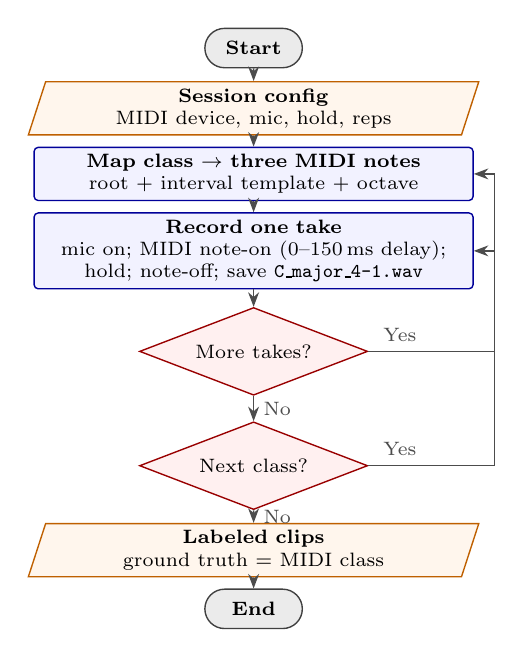
\begin{tikzpicture}[
    node distance=0.11cm and 0.10cm,
    >={Stealth},
    font=\scriptsize,
    base/.style={draw, align=center, minimum height=0.42cm, line width=0.5pt, inner sep=2.5pt},
    terminal/.style={base, shape=rounded rectangle, rounded rectangle arc length=180, draw=black!75, fill=black!8, minimum height=0.50cm, minimum width=1.8cm, inner xsep=8pt, font=\scriptsize\bfseries},
    process/.style={base, rectangle, rounded corners=1.5pt, draw=blue!60!black, fill=blue!5, text width=5.4cm},
    io/.style={base, trapezium, trapezium left angle=72, trapezium right angle=108, trapezium stretches body=true, draw=orange!75!black, fill=orange!7, text width=5.0cm, inner xsep=4pt},
    decision/.style={base, diamond, aspect=2.6, draw=red!60!black, fill=red!6, text width=2.2cm, inner sep=1pt},
    arrow/.style={->, line width=0.5pt, black!70}
  ]
    \node[terminal] (start) {Start};
    \node[io, below=0.16cm of start] (cfg)
    {\textbf{Session config}\\
     MIDI device, mic, hold, reps};
    \node[process, below=0.14cm of cfg] (map)
    {\textbf{Map class $\to$ three MIDI notes}\\
     root $+$ interval template $+$ octave};
    \node[process, below=0.14cm of map] (rec)
    {\textbf{Record one take}\\
     mic on; MIDI note-on (0--150\,ms delay);\\
     hold; note-off; save \texttt{C\_major\_4-1.wav}};
    \node[decision, below=0.22cm of rec] (morep)
    {More takes?};
    \node[decision, below=0.32cm of morep] (morec)
    {Next class?};
    \node[io, below=0.16cm of morec] (doneio)
    {\textbf{Labeled clips}\\
     ground truth $=$ MIDI class};
    \node[terminal, below=0.14cm of doneio] (endn) {End};
    \draw[arrow] (start) -- (cfg);
    \draw[arrow] (cfg) -- (map);
    \draw[arrow] (map) -- (rec);
    \draw[arrow] (rec) -- (morep);
    \draw[arrow] (morep.east) -- ++(1.6,0) node[above, font=\scriptsize, pos=0.25] {Yes}
      |- (rec.east);
    \draw[arrow] (morep) -- (morec) node[midway, right, font=\scriptsize] {No};
    \draw[arrow] (morec.east) -- ++(1.6,0) node[above, font=\scriptsize, pos=0.25] {Yes}
      |- (map.east);
    \draw[arrow] (morec) -- (doneio) node[midway, right, font=\scriptsize] {No};
    \draw[arrow] (doneio) -- (endn);
  \end{tikzpicture}%
  }
  \caption{Recorder loop. Class identity comes from the MIDI trigger, not from a human label after the fact.}
  \label{fig:esm-flow}
\end{figure}

Table~\ref{tab:esm-session} lists the session settings shared by every dataset.

\begin{table}[t]
\caption{Recorder session settings.}\label{tab:esm-session}
\begin{tabular}{@{}ll@{}}
\toprule
Parameter & Value \\
\midrule
Trigger & USB MIDI note-on (three notes) \\
Vocabulary & 12 roots $\times$ maj / min / dim, fourth octave \\
Voice & Grand-piano preset \\
Attack delay & 0--150\,ms (training) \\
Sample rate & 48{,}000\,Hz, mono \\
Training format & OGG/OPUS, 32-bit \\
Eval format & WAV \\
CQT window & first 2.0\,s of each clip \\
\bottomrule
\end{tabular}
\end{table}

\section{Dataset characteristics}\label{sec:datasets}

Table~\ref{tab:esm-inventory} is the inventory. Every dataset has all 36 classes and a constant take count (200 or 40). No class folder is missing. Durations sit above the 2.0\,s CQT crop. ThinkPad recordings are quieter than Vivo and Flow. Training CQT centroids sit higher ($\approx$467\,Hz) than the held-out sets ($\approx$269--323\,Hz).

Sixteen training clips are digital silence (peak $=0$), all of them $C$ diminished, which is 8\% of that class. They are what the \texttt{orig}/\texttt{clean} ablation removes. Vivo has 489 near-clip takes (hotter phone mic). No dataset has hard clipping.

\begin{table}[t]
\caption{Recorded datasets. Per-class count is constant. Duration and RMS are over all takes.}\label{tab:esm-inventory}
\setlength{\tabcolsep}{3.2pt}
\begin{tabular}{@{}llrrrrrr@{}}
\toprule
Dataset & Fmt & $N$ & /cls & Dur.\ min & Dur.\ mean & RMS dB & Cent.\ Hz \\
\midrule
\texttt{training} & OGG & 7{,}200 & 200 & 2.00 & 2.40 & $-21.4$ & 467 \\
\texttt{thinkpad} & WAV & 1{,}440 & 40 & 2.10 & 2.45 & $-26.6$ & 323 \\
\texttt{vivo} & WAV & 1{,}440 & 40 & 2.10 & 2.44 & $-19.2$ & 290 \\
\texttt{flow} & WAV & 1{,}440 & 40 & 2.10 & 2.44 & $-19.6$ & 269 \\
\texttt{thinkpad-2} & WAV & 1{,}440 & 40 & 2.16 & 2.52 & $-26.8$ & 310 \\
\texttt{flow-2} & WAV & 1{,}440 & 40 & 2.16 & 2.44 & $-22.6$ & 313 \\
\bottomrule
\end{tabular}
\end{table}

Fig.~\ref{fig:esm-chars} shows the same three quantities as distributions. Duration spread on \texttt{training} is the 0--150\,ms attack delay. The \texttt{thinkpad-2} tail above 3\,s is a longer hold, not a missing class. RMS separates the ThinkPad microphone from Vivo and Flow. Centroid separates the training tablet from every held-out microphone.

\begin{figure}[t]
\centering
\includegraphics[width=\textwidth]{esm-dataset-chars.pdf}
\caption{Dataset characteristics.
\textbf{(A)}~clip duration;
\textbf{(B)}~waveform RMS (training silence at $-240$\,dB clipped to $-40$ for display);
\textbf{(C)}~CQT spectral centroid.}
\label{fig:esm-chars}
\end{figure}

Fig.~\ref{fig:esm-cqt} is the mean CQT of each held-out dataset minus the training mean. Recording-setting datasets are cooler in the mid bins and hotter at the bottom. The two Yamaha datasets share a low-bin excess that the Techno recording-setting datasets do not, which is the keyboard factor visible in the feature the network reads.

\begin{figure}[t]
\centering
\includegraphics[width=\textwidth]{esm-cqt-shift.pdf}
\caption{Mean CQT difference: held-out mean minus training mean (dB). Same color scale on every panel.}
\label{fig:esm-cqt}
\end{figure}

\subsection{How much of the shift is a per-clip envelope offset}\label{sec:envelope}

Fig.~\ref{fig:esm-envelope} measures the shift in the two quantities a per-clip normalization would remove. Panel A is each clip's own dB mean over its $216\times188$ CQT. The held-out datasets sit between 8\,dB below (\texttt{vivo}, $-60.3$) and 7\,dB above (\texttt{thinkpad-2}, $-44.7$) the training mean of $-51.9$\,dB, so a large part of what changes with microphone or keyboard is a global level, not a change of shape.

Panel B decomposes each class centroid's drift from its training centroid into an offset component (what mean-centering removes), a scale component (what unit-normalizing removes), and a residual. Averaged over the 36 classes, the offset and scale terms together account for 31\% of the drift on \texttt{thinkpad}, 30\% on \texttt{flow}, 47\% on \texttt{flow-2}, 54\% on \texttt{thinkpad-2}, and 56\% on \texttt{vivo}. The residual is therefore the larger share on three of five datasets, which matters for Section~\ref{sec:baseline}: removing the offset does not have to remove most of the drift in order to fix the classification.

\begin{figure}[t]
\centering
\includegraphics[width=\textwidth]{esm-envelope-shift.pdf}
\caption{Envelope shift.
\textbf{(A)}~per-clip mean CQT level;
\textbf{(B)}~share of each class centroid's drift from training explained by a per-clip offset, a per-clip scale, and the residual.}
\label{fig:esm-envelope}
\end{figure}

\section{Training protocol and per-checkpoint record}\label{sec:training}

Every run was launched as its own operating-system process on one pinned RTX 2080 Ti with \texttt{TF\_DETERMINISTIC\_OPS=1} and batch size 32, so no two runs share a CUDA context and the spread reported below is not kernel-selection noise across devices. The seed sets the stratified 90/10 train/test split, the weight initialization, and the Python, NumPy, and TensorFlow global generators. Keras then reserves the last 10\% of the training partition for validation without re-stratifying, giving 81/9/10 overall.

Table~\ref{tab:esm-checkpoints} is the training record of all fifteen checkpoints. \texttt{EarlyStopping} has patience 6 and restores the best-validation-loss weights, so the restored epoch is always six less than the epochs run. Every \texttt{orig} run and four of five \texttt{clean} runs finish at 1.000 on their held-out in-domain split; \texttt{clean} seed 43 misses a single clip out of 719.

\begin{table}[t]
\caption{Per-checkpoint training record. \emph{Restored} is the epoch whose weights early stopping kept. In-domain accuracy is on each run's own held-out 10\% split. $^\dagger$Training-time collapse to chance, see Section~\ref{sec:insnorm}.}\label{tab:esm-checkpoints}
\setlength{\tabcolsep}{4pt}
\begin{tabular}{@{}llrrrrrr@{}}
\toprule
Variant & Seed & $N_{\text{train}}$ & $N_{\text{test}}$ & Epochs & Restored & Acc. & Macro F1 \\
\midrule
\texttt{orig} & 42 & 6{,}480 & 720 & 16 & 10 & 1.0000 & 1.0000 \\
\texttt{orig} & 43 & 6{,}480 & 720 & 24 & 18 & 1.0000 & 1.0000 \\
\texttt{orig} & 44 & 6{,}480 & 720 & 15 & 9 & 1.0000 & 1.0000 \\
\texttt{orig} & 45 & 6{,}480 & 720 & 14 & 8 & 1.0000 & 1.0000 \\
\texttt{orig} & 46 & 6{,}480 & 720 & 13 & 7 & 1.0000 & 1.0000 \\
\texttt{clean} & 42 & 6{,}465 & 719 & 10 & 4 & 1.0000 & 1.0000 \\
\texttt{clean} & 43 & 6{,}465 & 719 & 14 & 8 & 0.9986 & 0.9986 \\
\texttt{clean} & 44 & 6{,}465 & 719 & 14 & 8 & 1.0000 & 1.0000 \\
\texttt{clean} & 45 & 6{,}465 & 719 & 23 & 17 & 1.0000 & 1.0000 \\
\texttt{clean} & 46 & 6{,}465 & 719 & 21 & 15 & 1.0000 & 1.0000 \\
\texttt{insnorm} & 42 & 6{,}465 & 719 & 13 & 7 & 1.0000 & 1.0000 \\
\texttt{insnorm} & 43 & 6{,}465 & 719 & 7 & 1 & 0.0278$^\dagger$ & 0.0015$^\dagger$ \\
\texttt{insnorm} & 44 & 6{,}465 & 719 & 17 & 11 & 1.0000 & 1.0000 \\
\texttt{insnorm} & 45 & 6{,}465 & 719 & 16 & 10 & 1.0000 & 1.0000 \\
\texttt{insnorm} & 46 & 6{,}465 & 719 & 10 & 4 & 1.0000 & 1.0000 \\
\bottomrule
\end{tabular}
\end{table}

Fig.~\ref{fig:esm-history} shows the validation curves of the ten reported runs. Every run reaches 1.000 validation accuracy by epoch 2 or 3, so panel A separates nothing. Panel B does separate the runs, but not usefully: best validation loss ranges over six orders of magnitude, from $3\times10^{-9}$ to $1\times10^{-3}$, and its correlation with mean out-of-domain accuracy across the ten checkpoints is $-0.05$ (Pearson on $\log_{10}$ loss; Spearman $-0.01$). The restored epoch correlates at $r=0.36$. The two runs with the worst validation loss are \texttt{orig} seed 42 and \texttt{clean} seed 42, which are respectively the best and the worst out-of-domain checkpoints in the study. No quantity available at model-selection time predicts which checkpoint will transfer.

\begin{figure}[t]
\centering
\includegraphics[width=\textwidth]{esm-variant-history.pdf}
\caption{Validation curves of the ten reported checkpoints.
\textbf{(A)}~validation accuracy;
\textbf{(B)}~validation loss, log scale. The heavy line is \texttt{clean} seed 42, the earliest early stop and the worst out-of-domain run.}
\label{fig:esm-history}
\end{figure}

Table~\ref{tab:esm-kfold} and Fig.~\ref{fig:esm-kfold} are the five-fold in-domain cross-validation of Scenario~1, each fold retrained from a fresh initialization. Every fold reaches 1.000 test accuracy. Fig.~\ref{fig:esm-cm-train} is resubstitution on all 7{,}200 training takes, where one $C$ diminished take is labelled $C$ minor.

\begin{table}[t]
\caption{CNN in-domain 5-fold results.}\label{tab:esm-kfold}
\setlength{\tabcolsep}{3.5pt}
\begin{tabular}{@{}lrrrrrrr@{}}
\toprule
 & & \multicolumn{3}{c}{Accuracy} & \multicolumn{3}{c}{Loss} \\
\cmidrule(lr){3-5} \cmidrule(lr){6-8}
Fold & Ep. & Train & Val & Test & Train & Val & Test \\
\midrule
1 & 11 & 0.9979 & 1.000 & 1.000 & 0.0051 & 0.000 & 0.0003 \\
2 & 21 & 0.9979 & 1.000 & 1.000 & 0.0051 & 0.000 & 0.0000 \\
3 & 19 & 0.9969 & 1.000 & 1.000 & 0.0063 & 0.000 & 0.0000 \\
4 & 15 & 0.9967 & 1.000 & 1.000 & 0.0091 & 0.000 & 0.0000 \\
5 & 14 & 0.9985 & 1.000 & 1.000 & 0.0058 & 0.000 & 0.0001 \\
Mean & 16.0 & 0.9976 & 1.000 & 1.000 & 0.0074 & 0.000 & 0.0001 \\
\bottomrule
\end{tabular}
\end{table}

\begin{figure}[t]
\centering
\includegraphics[width=\textwidth]{esm-cnn-kfold.pdf}
\caption{Five-fold in-domain training.
\textbf{(A)}~accuracy (solid train, dashed val);
\textbf{(B)}~train loss.}
\label{fig:esm-kfold}
\end{figure}

\begin{figure}[t]
\centering
\includegraphics[width=0.88\textwidth,height=0.55\textheight,keepaspectratio]{esm-cm-training.pdf}
\caption{Training-set confusion matrix (7{,}200 takes, 200 per class). Off-diagonal mass is one $C$ dim $\to$ $C$ min.}
\label{fig:esm-cm-train}
\end{figure}

\section{Recorded out-of-domain results, per checkpoint}\label{sec:recorded}

Fig.~\ref{fig:esm-seed-spread} places all fifteen checkpoints on the five recorded held-out datasets. The vertical extent of each cluster, not its mean, is the object of the main article: on \texttt{thinkpad-2} the ten reported checkpoints run from 0.348 to 0.963.

\begin{figure}[t]
\centering
\includegraphics[width=\textwidth]{esm-seed-spread.pdf}
\caption{Accuracy of every checkpoint on the five recorded held-out datasets. Dashes are per-variant means; the hollow marker is \texttt{insnorm} seed 43, excluded from its mean. The dashed line is the zero-parameter centroid baseline of Section~\ref{sec:baseline}, and the cross is the earlier single checkpoint of Section~\ref{sec:provenance}.}
\label{fig:esm-seed-spread}
\end{figure}

Table~\ref{tab:esm-factors} expands the factor ranking of the main article into all twenty comparisons. The keyboard gap is the Techno accuracy minus the matched Yamaha accuracy on the same checkpoint and recording setting; the recording-setting cost is $1.000$ minus that same Techno accuracy. The gap is positive on all twenty rows. It exceeds the recording-setting cost on eighteen of them, and the two exceptions are both on the Flow pair with an unusually weak Techno baseline. Five rows have the two costs within 3 points of each other and are not resolved by datasets of this size.

\begin{table}[t]
\caption{All twenty matched factor comparisons, in accuracy points. \emph{Gap} is the keyboard cost, \emph{RS} the recording-setting cost. $^\ast$Recording setting is the larger factor. $^\circ$The two costs differ by less than 3 points.}\label{tab:esm-factors}
\setlength{\tabcolsep}{4pt}
\begin{tabular}{@{}llrrrrl@{}}
\toprule
Variant & Seed & Pair & Techno & Yamaha & Gap & RS \\
\midrule
\texttt{orig} & 42 & ThinkPad & 0.999 & 0.963 & 3.6 & 0.1 \\
\texttt{orig} & 42 & Flow & 0.994 & 0.961 & 3.3 & 0.6$^\circ$ \\
\texttt{orig} & 43 & ThinkPad & 0.967 & 0.719 & 24.8 & 3.3 \\
\texttt{orig} & 43 & Flow & 0.862 & 0.720 & 14.2 & 13.8$^\circ$ \\
\texttt{orig} & 44 & ThinkPad & 0.958 & 0.847 & 11.1 & 4.2 \\
\texttt{orig} & 44 & Flow & 0.940 & 0.842 & 9.8 & 6.0 \\
\texttt{orig} & 45 & ThinkPad & 0.895 & 0.705 & 19.0 & 10.5 \\
\texttt{orig} & 45 & Flow & 0.801 & 0.740 & 6.0 & 19.9$^\ast$ \\
\texttt{orig} & 46 & ThinkPad & 0.984 & 0.780 & 20.4 & 1.6 \\
\texttt{orig} & 46 & Flow & 0.958 & 0.810 & 14.7 & 4.2 \\
\texttt{clean} & 42 & ThinkPad & 0.985 & 0.348 & 63.8 & 1.5 \\
\texttt{clean} & 42 & Flow & 0.831 & 0.368 & 46.3 & 16.9 \\
\texttt{clean} & 43 & ThinkPad & 0.857 & 0.698 & 15.9 & 14.3$^\circ$ \\
\texttt{clean} & 43 & Flow & 0.810 & 0.685 & 12.6 & 19.0$^\ast$ \\
\texttt{clean} & 44 & ThinkPad & 0.975 & 0.925 & 5.0 & 2.5$^\circ$ \\
\texttt{clean} & 44 & Flow & 0.981 & 0.935 & 4.7 & 1.9$^\circ$ \\
\texttt{clean} & 45 & ThinkPad & 0.999 & 0.884 & 11.5 & 0.1 \\
\texttt{clean} & 45 & Flow & 0.988 & 0.903 & 8.5 & 1.2 \\
\texttt{clean} & 46 & ThinkPad & 0.996 & 0.740 & 25.6 & 0.4 \\
\texttt{clean} & 46 & Flow & 0.891 & 0.749 & 14.2 & 10.9 \\
\bottomrule
\end{tabular}
\end{table}

\section{Eval-only overlays}\label{sec:overlays}

\subsection{Bank construction}\label{sec:banks}

\emph{Noise.} 400 ESC-50 clips \cite{Piczak2015}, the complete interior and domestic group: \texttt{can\_opening}, \texttt{clock\_alarm}, \texttt{clock\_tick}, \texttt{door\_wood\_creaks}, \texttt{door\_wood\_knock}, \texttt{glass\_breaking}, \texttt{keyboard\_typing}, \texttt{mouse\_click}, \texttt{vacuum\_cleaner}, \texttt{washing\_machine}, 40 clips each. Each is reduced to a 2.0\,s segment of maximum energy and converted to a $216\times188$ CQT under the same hop and binning as the chord features. Mixing is in the CQT power domain, one noise matrix per chord clip at a broadband SNR drawn uniformly from $[10,25]$\,dB, with the noise matrix rolled in time by a random offset.

\emph{Room impulse responses.} The IR Survey \cite{Traer2016} contributes 174 responses spanning 51 indoor room types (bedrooms, classrooms, offices, kitchens, halls, galleries, and similar), after removing bathrooms, showers, outdoor and semi-outdoor spaces, and vehicles and transit stations. Responses are made mono, resampled to 48\,kHz, trimmed of leading silence below $-40$\,dB relative to peak, and peak-normalized. Durations run 0.18--1.99\,s, median 0.62\,s.

\emph{Microphone impulse responses.} Six measured vintage-capsule responses: AKG D12, Crystal, Lomo 52A5M, Melodium RM6, Oktava MD57, and STC 4035, each 0.5\,s, prepared identically to the room bank.

Both impulse-response banks convolve the evaluation waveform before CQT extraction, one response drawn per clip, with a fixed draw seed. Nothing is written back into training, and the overlays are applied to the five held-out datasets only. A set of feature-faithful audio renderings, one per overlay for fifteen clips across three datasets with a manifest naming the drawn impulse response, noise file, SNR, and time offset, accompanies this supplement so the overlays can be listened to rather than only read.

Fig.~\ref{fig:esm-overlay-cqt} shows one clip under each overlay in the CQT the network actually sees. Noise fills the gaps between partials, the room response smears energy across frames, and the microphone response darkens the low bins as a spectral tilt without adding a partial. That last panel is the visual form of the result in Section~\ref{sec:overlay-results}: a capsule response moves the level, not the interval structure.

\begin{figure}[t]
\centering
\includegraphics[width=\textwidth]{esm-overlay-cqt.pdf}
\caption{One \texttt{vivo} take of $C$ maj (top) and $E$ dim (bottom) after each eval-only overlay. These are the stored CQT matrices, not time-domain mixes.}
\label{fig:esm-overlay-cqt}
\end{figure}

\subsection{Per-checkpoint overlay results}\label{sec:overlay-results}

The main article gives every seed under noise and reports only means for the other two overlays. Tables~\ref{tab:esm-rir} and~\ref{tab:esm-dir} give the room and microphone responses per checkpoint, and Fig.~\ref{fig:esm-overlay-tax} plots all three taxes together.

\begin{table}[t]
\caption{Accuracy under eval-only indoor room impulse responses, per checkpoint.}\label{tab:esm-rir}
\setlength{\tabcolsep}{4pt}
\begin{tabular}{@{}llrrrrr@{}}
\toprule
Variant & Seed & \texttt{thinkpad} & \texttt{vivo} & \texttt{flow} & \texttt{thinkpad-2} & \texttt{flow-2} \\
\midrule
\texttt{orig} & 42 & 0.963 & 0.964 & 0.979 & 0.908 & 0.919 \\
\texttt{orig} & 43 & 0.882 & 0.811 & 0.833 & 0.644 & 0.659 \\
\texttt{orig} & 44 & 0.869 & 0.778 & 0.892 & 0.783 & 0.766 \\
\texttt{orig} & 45 & 0.782 & 0.706 & 0.769 & 0.563 & 0.598 \\
\texttt{orig} & 46 & 0.954 & 0.891 & 0.936 & 0.775 & 0.791 \\
\texttt{orig} & Mean & 0.890 & 0.830 & 0.882 & 0.735 & 0.747 \\
\texttt{clean} & 42 & 0.849 & 0.783 & 0.810 & 0.361 & 0.382 \\
\texttt{clean} & 43 & 0.767 & 0.660 & 0.811 & 0.631 & 0.605 \\
\texttt{clean} & 44 & 0.928 & 0.863 & 0.942 & 0.840 & 0.854 \\
\texttt{clean} & 45 & 0.964 & 0.947 & 0.970 & 0.871 & 0.883 \\
\texttt{clean} & 46 & 0.879 & 0.780 & 0.851 & 0.624 & 0.631 \\
\texttt{clean} & Mean & 0.877 & 0.806 & 0.877 & 0.666 & 0.671 \\
\bottomrule
\end{tabular}
\end{table}

\begin{table}[t]
\caption{Accuracy under eval-only measured microphone impulse responses, per checkpoint.}\label{tab:esm-dir}
\setlength{\tabcolsep}{4pt}
\begin{tabular}{@{}llrrrrr@{}}
\toprule
Variant & Seed & \texttt{thinkpad} & \texttt{vivo} & \texttt{flow} & \texttt{thinkpad-2} & \texttt{flow-2} \\
\midrule
\texttt{orig} & 42 & 0.986 & 0.995 & 0.997 & 0.942 & 0.951 \\
\texttt{orig} & 43 & 0.962 & 0.892 & 0.920 & 0.664 & 0.706 \\
\texttt{orig} & 44 & 0.956 & 0.907 & 0.957 & 0.833 & 0.832 \\
\texttt{orig} & 45 & 0.926 & 0.846 & 0.892 & 0.632 & 0.683 \\
\texttt{orig} & 46 & 0.965 & 0.972 & 0.985 & 0.777 & 0.797 \\
\texttt{orig} & Mean & 0.959 & 0.922 & 0.950 & 0.770 & 0.794 \\
\texttt{clean} & 42 & 0.961 & 0.872 & 0.904 & 0.330 & 0.345 \\
\texttt{clean} & 43 & 0.835 & 0.771 & 0.863 & 0.606 & 0.622 \\
\texttt{clean} & 44 & 0.961 & 0.959 & 0.978 & 0.887 & 0.908 \\
\texttt{clean} & 45 & 0.994 & 0.994 & 0.974 & 0.877 & 0.897 \\
\texttt{clean} & 46 & 0.945 & 0.882 & 0.904 & 0.637 & 0.693 \\
\texttt{clean} & Mean & 0.939 & 0.895 & 0.925 & 0.667 & 0.693 \\
\bottomrule
\end{tabular}
\end{table}

\begin{figure}[t]
\centering
\includegraphics[width=\textwidth]{esm-overlay-tax.pdf}
\caption{Overlay tax per checkpoint, recorded accuracy minus overlay accuracy.
\textbf{(A)}~ESC-50 interior noise;
\textbf{(B)}~indoor room impulse response;
\textbf{(C)}~measured microphone impulse response. Dashes are per-variant means. Negative values are overlays that helped.}
\label{fig:esm-overlay-tax}
\end{figure}

Two features of Fig.~\ref{fig:esm-overlay-tax} are worth stating explicitly. First, the noise tax is larger on the two Yamaha datasets than on the three Techno ones for \texttt{orig} (15.3 and 14.5 points against 10.2, 7.6, and 6.5) but not for \texttt{clean} (10.5 on both Yamaha sets against 8.7, 8.5, and 7.3), so the compounding of noise with keyboard shift is clear in one variant and flat in the other. Second, the microphone tax straddles zero: it is negative on \texttt{vivo} and \texttt{flow} for \texttt{orig} ($-2.0$ and $-3.9$ points, meaning the convolved audio scored \emph{higher} than the recording), and positive but small on the Yamaha sets. Averaged over the three Techno datasets it is $-1.9$ points on \texttt{orig} and $-0.1$ on \texttt{clean}, against 7.5--8.1 points for an actual change of microphone. Convolution with a capsule response is not a substitute for recording through a different device, and on these checkpoints it is not even reliably a degradation.

\section{Where the error lands}\label{sec:perclass}

Table~\ref{tab:esm-quality} is per-quality recall averaged over the five seeds of each variant. Diminished triads, the closest-packed template, are the weakest quality on both Yamaha datasets under both variants, and are already the weakest on \texttt{vivo} under a recording-setting change alone.

\begin{table}[t]
\caption{Recall by chord quality, mean over the five seeds of each variant.}\label{tab:esm-quality}
\setlength{\tabcolsep}{5pt}
\begin{tabular}{@{}llrrr@{}}
\toprule
Variant & Dataset & Major & Minor & Dim \\
\midrule
\texttt{orig} & \texttt{thinkpad} & 0.989 & 0.930 & 0.963 \\
\texttt{orig} & \texttt{vivo} & 0.978 & 0.903 & 0.827 \\
\texttt{orig} & \texttt{flow} & 0.954 & 0.897 & 0.882 \\
\texttt{orig} & \texttt{thinkpad-2} & 0.835 & 0.843 & 0.730 \\
\texttt{orig} & \texttt{flow-2} & 0.827 & 0.857 & 0.760 \\
\texttt{clean} & \texttt{thinkpad} & 0.951 & 0.973 & 0.963 \\
\texttt{clean} & \texttt{vivo} & 0.913 & 0.900 & 0.870 \\
\texttt{clean} & \texttt{flow} & 0.914 & 0.898 & 0.890 \\
\texttt{clean} & \texttt{thinkpad-2} & 0.740 & 0.778 & 0.639 \\
\texttt{clean} & \texttt{flow-2} & 0.736 & 0.800 & 0.648 \\
\bottomrule
\end{tabular}
\end{table}

Which \emph{individual} classes fail is not stable across seeds, and this is the main correction the per-seed protocol makes to a single-run reading. Table~\ref{tab:esm-zero} counts, for each variant and dataset, how many of the 36 classes reach zero recall on at least one seed and how many (class, seed) cells that involves. On \texttt{orig}/\texttt{thinkpad-2}, eleven different classes hit zero on at least one of five seeds, and no class hits zero on more than three. Both Techno ThinkPad columns are empty: no class collapses there in any run. The earlier single checkpoint of Section~\ref{sec:provenance} showed zero recall on $D$ minor, $E$ diminished, and $G\sharp$ diminished; across the ten reported checkpoints those three are unremarkable, and a per-class error story told from one run would have named the wrong classes.

\begin{table}[t]
\caption{Zero-recall incidence across the five seeds of each variant. \emph{Classes} is how many of the 36 reach zero recall on at least one seed; \emph{cells} is the number of (class, seed) pairs at zero.}\label{tab:esm-zero}
\setlength{\tabcolsep}{5pt}
\begin{tabular}{@{}lrrrr@{}}
\toprule
 & \multicolumn{2}{c}{\texttt{orig}} & \multicolumn{2}{c}{\texttt{clean}} \\
\cmidrule(lr){2-3} \cmidrule(lr){4-5}
Dataset & Classes & Cells & Classes & Cells \\
\midrule
\texttt{thinkpad} & 0 & 0 & 0 & 0 \\
\texttt{vivo} & 5 & 8 & 5 & 6 \\
\texttt{flow} & 4 & 4 & 7 & 8 \\
\texttt{thinkpad-2} & 11 & 15 & 19 & 24 \\
\texttt{flow-2} & 8 & 8 & 15 & 20 \\
\bottomrule
\end{tabular}
\end{table}

\subsection{Anatomy of the \texttt{clean} seed-42 collapse}\label{sec:collapse}

The worst checkpoint in the study is worth describing in detail, because 0.348 accuracy could mean many different things. On \texttt{thinkpad-2}, that checkpoint predicts only 21 of the 36 classes and routes 358 of 1{,}440 clips to $C$ minor, the same class the single resubstitution error falls into. It keeps the correct root on 46.7\% of clips and the correct quality on 58.1\%, so at 0.348 it is running at about 12.5 times chance: degraded, not dead, and still carrying most of the harmonic information in its errors. Its training log is unremarkable except for finishing earliest of the ten, restored from epoch 4 against a next-earliest of 7, and, as Section~\ref{sec:training} shows, the restored epoch explains little across the ten runs ($r=0.36$). The same seed under \texttt{orig} is the best out-of-domain checkpoint in the study, and the two runs do not share a data partition, so nothing here attributes the collapse to the sixteen silent clips on their own.

\section{Third variant: per-sample input normalization}\label{sec:insnorm}

The main article's architecture normalizes the input with a batch-normalization layer on the frequency axis, which fits one scale and shift per CQT bin to the Techno training distribution and then applies that fixed transform to every clip at inference. The \texttt{insnorm} variant replaces that layer with a per-sample standardization, subtracting each clip's own mean and dividing by its own standard deviation over the whole $216\times188$ plane. Everything else, including the training pool of 7{,}184 clips, the seeds, and every hyperparameter, is identical to \texttt{clean}.

Table~\ref{tab:esm-insnorm} gives its out-of-domain accuracy. Excluding its collapsed seed, it is the strongest variant on every recorded dataset, and by a wide margin where the main article's gap is largest: 0.907 and 0.917 on the two Yamaha datasets against 0.803 / 0.815 for \texttt{orig} and 0.719 / 0.728 for \texttt{clean}. Seed 46 reaches 0.992 and 0.995 there. Its overlay means are correspondingly high, 0.866 / 0.880 on the Yamaha datasets under noise where \texttt{orig} manages 0.650 / 0.670.

\begin{table}[t]
\caption{\texttt{insnorm} out-of-domain accuracy per seed, and overlay means. Seed 43 collapsed during training and is excluded from the summary rows.}\label{tab:esm-insnorm}
\setlength{\tabcolsep}{4pt}
\begin{tabular}{@{}lrrrrr@{}}
\toprule
Seed & \texttt{thinkpad} & \texttt{vivo} & \texttt{flow} & \texttt{thinkpad-2} & \texttt{flow-2} \\
\midrule
42 & 0.999 & 1.000 & 0.997 & 0.942 & 0.944 \\
43 & 0.028 & 0.028 & 0.028 & 0.028 & 0.028 \\
44 & 0.997 & 0.997 & 0.998 & 0.881 & 0.892 \\
45 & 0.907 & 0.958 & 0.976 & 0.815 & 0.835 \\
46 & 1.000 & 1.000 & 1.000 & 0.992 & 0.995 \\
\midrule
Mean & 0.976 & 0.989 & 0.993 & 0.907 & 0.917 \\
SD & 0.046 & 0.021 & 0.011 & 0.077 & 0.069 \\
\midrule
Noise & 0.937 & 0.934 & 0.949 & 0.866 & 0.880 \\
Room IR & 0.959 & 0.976 & 0.972 & 0.876 & 0.894 \\
Mic IR & 0.984 & 0.996 & 0.996 & 0.923 & 0.930 \\
\bottomrule
\end{tabular}
\end{table}

That result comes with a failure mode the other two variants do not have. \texttt{insnorm} seed 43 never leaves chance: its loss sits at $\ln 36$ from the first epoch, early stopping restores epoch 1, and it scores 0.0278 both in domain and on every held-out dataset. Retraining reproduces it identically, so it is a deterministic property of that seed under this normalization rather than transient noise, and a control run with the standardization epsilon raised to $10^{-3}$ reproduced it as well. Where the \texttt{clean} seed-42 collapse of Section~\ref{sec:collapse} is invisible in domain and appears only under shift, this one is visible immediately.

We report \texttt{insnorm} here rather than in the main article because it changes the architecture rather than the training set, so it is not part of the data-quality ablation, and because four usable seeds are a thin basis for a variant recommendation. It is, however, the strongest available evidence about mechanism: replacing a normalization fitted once to the training distribution with one computed per clip recovers most of the keyboard gap the main article measures, which is what the envelope measurements of Section~\ref{sec:envelope} and the baseline of Section~\ref{sec:baseline} would predict.

\section{A zero-parameter nearest-centroid baseline}\label{sec:baseline}

Nothing in the main article establishes that the recorded shifts are hard for a classifier in general, only that they are expensive for this network. A nearest-centroid classifier on the identical CQT features settles that question, and it settles it in an uncomfortable direction.

The classifier stores 36 class means from the training features and assigns each evaluation clip to the nearest mean. It has no learned parameters, no seed, and no training run. Five distance definitions isolate what normalization is doing:

\begin{description}
\item[Raw distance] squared Euclidean distance on the dB-CQT.
\item[Scale only] each clip divided by its own standard deviation, then Euclidean.
\item[Centering only] each clip's own mean subtracted, then Euclidean.
\item[Cosine, no centering] $L_2$-normalized, then cosine similarity.
\item[Centering $+$ scale] mean-subtracted and $L_2$-normalized, then cosine, that is, correlation distance.
\end{description}

In domain, stratified five-fold on the training set gives 0.9996 mean accuracy on the 7{,}184-clip pool under both the Euclidean and the correlation metric, and 0.9974--0.9976 with the sixteen silent clips included: essentially the same in-domain ceiling as the CNN, from 36 stored means.

Out of domain, Table~\ref{tab:esm-baseline} is the result. Correlation distance scores \textbf{1.0000 on all five recorded datasets}, including both Yamaha keyboard-shift sets where the ten CNN checkpoints average 0.72--0.82 and range down to 0.348. It also scores 0.9986--1.0000 under all three eval-only overlays on all five datasets. The margin is not marginal: the cosine similarity to the true class centroid exceeds the best wrong centroid on every one of the 7{,}200 held-out clips, with a median margin of 0.098--0.122 and a minimum of 0.024.

\begin{table}[t]
\caption{Nearest-centroid accuracy, 36 class means fitted on the 7{,}184 non-silent training clips. Recorded datasets (top) and eval-only overlays, mean over the five datasets (bottom).}\label{tab:esm-baseline}
\setlength{\tabcolsep}{3.6pt}
\begin{tabular}{@{}lrrrrr@{}}
\toprule
Metric & \texttt{thinkpad} & \texttt{vivo} & \texttt{flow} & \texttt{thinkpad-2} & \texttt{flow-2} \\
\midrule
Raw distance & 1.0000 & 0.8910 & 0.9993 & 0.8590 & 0.9181 \\
Scale only & 0.9931 & 0.9986 & 0.9882 & 0.9986 & 0.9979 \\
Centering only & 1.0000 & 1.0000 & 1.0000 & 1.0000 & 1.0000 \\
Cosine, no cent. & 0.9979 & 1.0000 & 1.0000 & 1.0000 & 1.0000 \\
Centering $+$ scale & 1.0000 & 1.0000 & 1.0000 & 1.0000 & 1.0000 \\
\midrule
\multicolumn{6}{@{}l}{\textit{Noise}} \\
Raw distance & 0.8403 & 0.9201 & 0.8833 & 0.5361 & 0.5646 \\
Centering $+$ scale & 0.9986 & 1.0000 & 1.0000 & 1.0000 & 1.0000 \\
\multicolumn{6}{@{}l}{\textit{Room IR}} \\
Raw distance & 0.9868 & 0.7986 & 0.9694 & 0.9076 & 0.9417 \\
Centering $+$ scale & 1.0000 & 1.0000 & 1.0000 & 1.0000 & 1.0000 \\
\multicolumn{6}{@{}l}{\textit{Mic IR}} \\
Raw distance & 0.9563 & 0.8104 & 0.9639 & 0.9653 & 0.9896 \\
Centering $+$ scale & 1.0000 & 1.0000 & 1.0000 & 1.0000 & 1.0000 \\
\bottomrule
\end{tabular}
\end{table}

Fig.~\ref{fig:esm-baseline} shows which step buys this. Removing the per-clip mean is the whole effect: centering alone reaches 1.0000 everywhere, scale alone does not (0.51--0.56 on the Yamaha datasets under the microphone overlay), and raw distance gives up as much as 46 points, worst on \texttt{thinkpad-2} under noise (0.536). The classifier is not solving the shift; it is discarding the dimension along which the shift mostly lies. Section~\ref{sec:envelope} measured that dimension directly and found that offset and scale explain only 30--56\% of each class centroid's drift, so the residual 44--70\% is real but evidently does not reorder the 36 centroids.

\begin{figure}[t]
\centering
\includegraphics[width=\textwidth]{esm-baseline-metrics.pdf}
\caption{Nearest-centroid accuracy by distance definition.
\textbf{(A)}~recorded held-out datasets;
\textbf{(B)}~eval-only overlays, averaged over the five datasets.}
\label{fig:esm-baseline}
\end{figure}

A coarser representation is not what carries this. Folding the same CQT bins down to twelve pitch classes and matching centroids reaches 0.98--1.00 on all five datasets in the dB domain, but only 0.42--0.93 if the fold is done in the power domain, the difference again being whether a per-clip level survives into the representation.

Three consequences follow, and they qualify the main article rather than contradict it.

First, the 36-class isolated-triad problem posed by these recordings is not intrinsically difficult under any of the shifts tested. Everything the CNN loses out of domain is lost to something other than the discriminability of the classes.

Second, the ranking the main article reports, keyboard above recording setting, is a property of this network under this normalization, not of the acoustic shifts themselves. A classifier that removes the per-clip envelope sees no ordering at all because it sees no cost at all.

Third, the mechanism the main article infers from the error structure, that a keyboard change moves the spectral envelope more than the interval spacing, is supported from the other side here: a method that removes exactly the envelope removes exactly the gap, and the \texttt{insnorm} variant of Section~\ref{sec:insnorm} recovers most of it inside the network.

The baseline's own limits should be read alongside this. It is fitted and tested on isolated, fixed-length, single-voicing triads with one note onset per clip, which is the regime in which a class mean is a sufficient statistic. It has no path to polyphonic or continuous audio, no time model, and no capacity for the vocabularies the chord-recognition literature actually targets. What it establishes is a floor for this dataset, not an alternative to learned models on the task at large.

\section{Reproducibility}\label{sec:repro}

Software: Python 3.10, TensorFlow 2.15, scikit-learn 1.7.2, Librosa 0.11.0, NumPy 1.26.4, Matplotlib 3.10.8. Training ran on one pinned RTX 2080 Ti with \texttt{TF\_DETERMINISTIC\_OPS=1}, one operating-system process per run. Feature extraction and evaluation used a ROG Flow X13 (Ryzen 7 6800HS, 16\,GB RAM) and Google Colaboratory (T4/A100).

CQT extraction is identical for training, every recorded dataset, and every overlay: \texttt{librosa.cqt()} at 48\,kHz, hop 512, Hann window, 6 octaves from C1 at 36 bins per octave, first 2.0\,s of each clip, magnitudes to dB with \texttt{amplitude\_to\_db(ref=max)}, stored as $216\times188\times1$.

The recorded datasets are at \url{https://zenodo.org/records/21077144} and the recording tool at \url{https://github.com/sglkc/chords-dataset-generator/}. Per-checkpoint outputs referenced above are the training record (\texttt{progress.csv}), the per-epoch curves (\texttt{history/}), the recorded and overlay accuracies (\texttt{pooled\_ood\_seeds.csv}, \texttt{overlay\_pooled\_seeds.csv}), the per-class recall of all fifteen checkpoints (\texttt{per\_class\_recall\_seeds.csv}), and the baseline results (\texttt{summary.csv}, \texttt{overlay\_summary.csv}, \texttt{envelope\_drift\_decomposition.csv}, \texttt{rank1\_margins.csv}), all in the project repository alongside the notebooks that wrote them.

\bibliography{mendeley}

\end{document}
